
\section[Implementaci\'on de arquitectura de software del controlador]
		{Implementaci\'on de arquitectura de software del controlador}
La implementaci\'on de la arquitectura de software del controlador la hicimos en C++, tal
como explicamos en la secci\'on \ref{interfaces}. La relaci\'on explicada en dicha secci\'on
entre el robot(con sus dispositivos), los comportamientos y el sistema de reconocimiento se
puede ver m\'as claramente en la figura\ref{fig:theAllTogether}, unidos por la clase \textit{GarbageCleaner},
que implementa la arquitectura \emph{Subsumption}. En la misma tambi\'en est\'a el main-loop. Mostramos
en la figura \ref{fig:soft_arq_behaviours} que \textit{GarbageCleaner} posee comportamientos, as\'i como tambi\'en
un robot y el mismo posee dispositivos que pueden ser sensores o actuadores, tal como se ve
en la figura \ref{fig:soft_arq_devices}. Tambi\'en posee el m\'odulo de reconocimiento de
objetos, mostrado en la figura \ref{fig:soft_arq_reconmodule}. La implementaci\'on de \textit{GarbageCleaner}
es simple, ya que debe:
\begin{itemize}
	\item{} Obtener los sensores y actuadores del robot.
	\item{} Inicializar el m\'odulo de reconocimiento de basuras.
	\item{} Instanciar los comportamientos, brind\'andoles los sensores, actuadores y eventualmente
			el m\'odulo de reconocimiento, necesarios para saber si su est\'imulo est\'a activo y
			para poder interactuar con el entorno.
	\item{} Correr el main-loop, utilizando la arquitectura de comportamientos
			elegida(\emph{Subsumption}), haciendo actuar al comportamiento cuyo est\'imulo
			est\'e activo en ese instante de tiempo y tenga mayor nivel en la arquitectura.
\end{itemize}
\begin{landscape}
\begin{figure}[h]
	\centering
	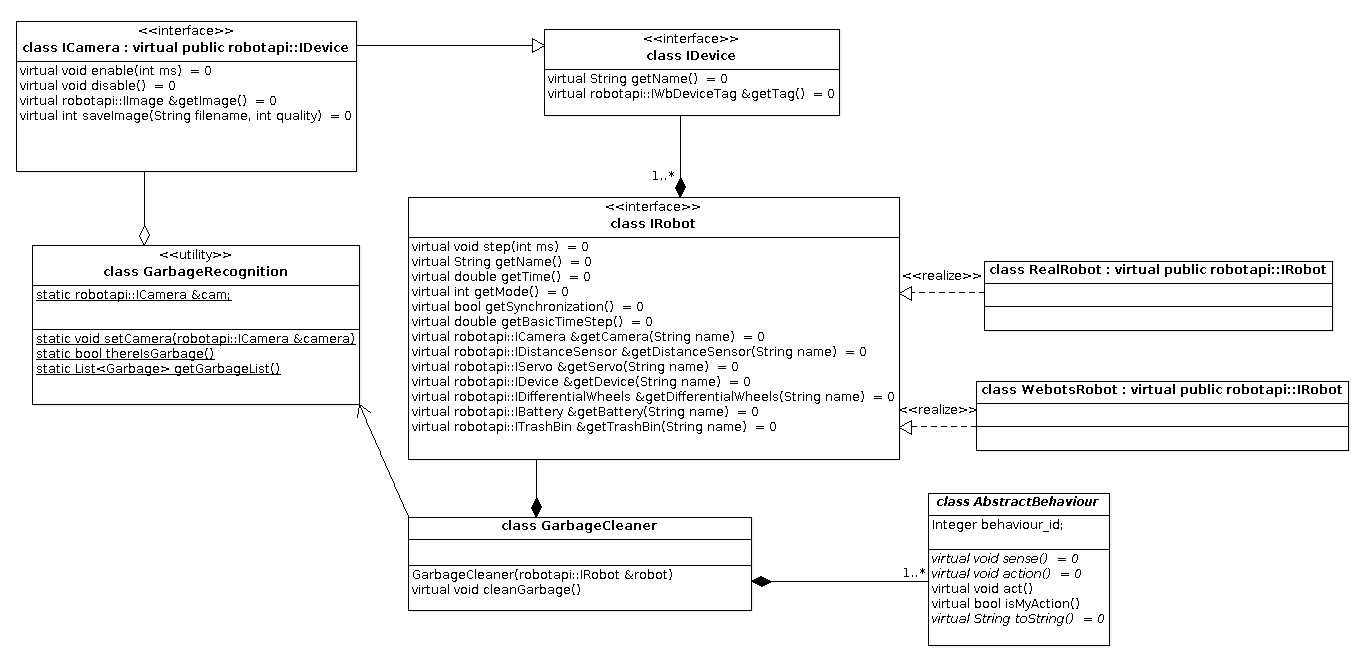
\includegraphics[scale=0.52]{comportamientos/figures/api4.png}
	\caption[Arquitectura de software: principales componentes]{Diagrama de clases de la arquitectura
			de sofware. Relaci\'on entre las 3 grandes componentes del proyecto}
	\label{fig:theAllTogether}
\end{figure}
\end{landscape}

\subsection{Comportamientos}
Como ya mencionamos anteriormente, en la figura \ref{fig:soft_arq_behaviours} mostramos la
relaci\'on de \textit{GarbageCleaner} con los comportamientos. Podemos ver que m\'as precisamente posee
 \textit{AbstractBehaviours}. \'Esto se debe a que la \'unica informaci\'on que necesita para coordinarlos
es saber si est\'an activos (m\'etodo \textit{sense}) y luego poder indicarles que den su respuesta
(m\'etodo \textit{act}).
\\\indent
Para agregar un comportamiento, es necesario que extienda de \textit{AbstractBehaviour} e implemente
los m\'etodos abstractos de la clase: \textit{sense}, \textit{action} y \textit{toString}. En el primero el comportamiento
debe indicar si est\'a activo o no en base a la informaci\'on de los sensores que utilice. En el
segundo se debe implementar la respuesta del comportamiento en el caso que est\'e activo. El
\'ultimo m\'etodo provee una descripci\'on del comportamiento implementado. Finalmente, hay
que instanciarlo y agregarlo a la lista de comportamientos que posee \textit{GarbageCleaner}.
\begin{landscape}
\begin{figure}[h]
	\centering
	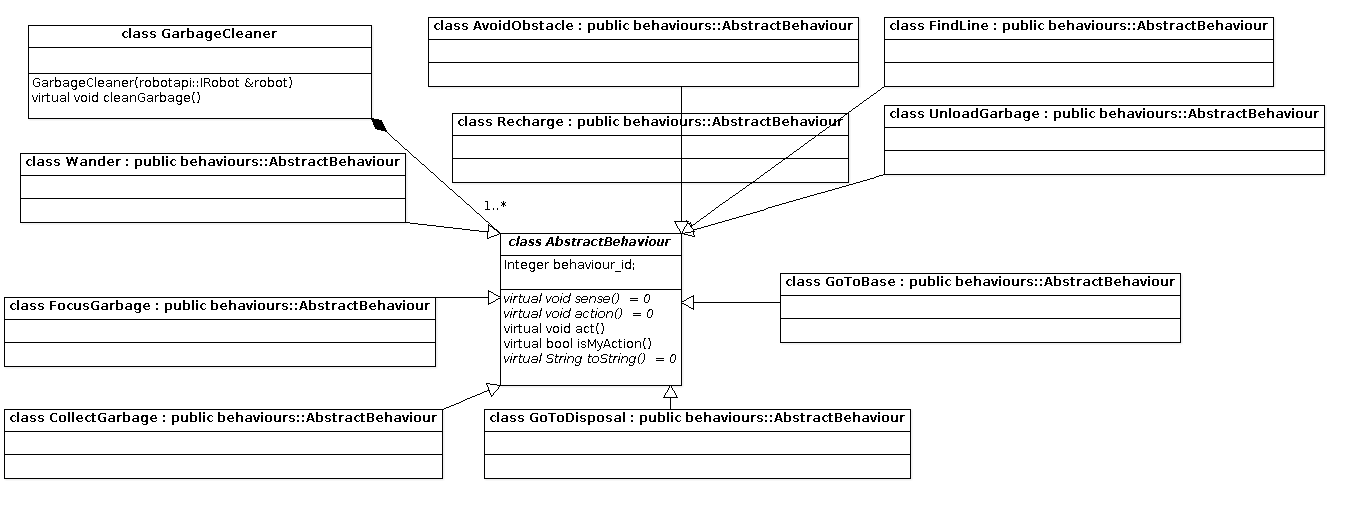
\includegraphics[scale=0.52]{comportamientos/figures/api1.png}
	\caption[Arquitectura de software: comportamientos]{Diagrama de clases de la arquitectura
			de sofware. Paquete de comportamientos}
	\label{fig:soft_arq_behaviours}
\end{figure}
\end{landscape}

\subsection{Dispositivos del robot}
Para que los comportamientos sensen y act\'uen con el entorno, deben disponer de dispositivos
que les permitan hacerlo. \'Estos \'ultimos forman parte del \textit{IRobot} que le es entregado a
 \textit{GarbageCleaner} para que instancie los comportamientos. Como se puede observar, la
interfaz que representa al robot provee m\'etodos de obtenci\'on de sensores como \textit{getDistanceSensor}
y de actuadores, como \textit{getDifferentialWheels}. Para el desarrollo de la arquitectura nos basamos
fuertemente en la api que provee Webots para interactuar con su robot simulado.
\\\indent
Para minimizar el acoplamiento entre \textit{IRobot} y \textit{GarbageCleaner}, hicimos que los dispositivos
sean pedidos por un nombre que los representa. En la implementaci\'on de la interfaz para la simulaci\'on
con Webots (\textit{WebotsRobot}), la mayor cantidad de llamadas a \'estos m\'etodos son simples wrappers
de una invocaci\'on al dispositivo virtual del programa de simulaci\'on. La implementaci\'on para el robot
real, \textit{RealRobot}, posee un mapa que relaciona los nombres de los dispositivos con instancias de
implementaciones de los mismos. \'Estas implementaciones, como por ejemplo \textit{RealDistanceSensor},
tienen los handlers necesarios para poder enviar y recibir informaci\'on de los sensores y actuadores de
los cuales son responsables. En el caso de \textit{RealDifferentialWheels}, el mismo posee dos handlers,
dado que cada handler es capaz de interactuar con una placa con determinado groupid y boardid, y cada
motor posee una placa que lo controla.
\\\indent
En el caso que se quiera agregar un sensor nuevo a la api, como por ejemplo un GPS, es necesario
crear la interfaz que represente el mismo, con m\'etodos de obtenci\'on de valores de los sensores o
seteo de valores para los actuadores. Luego de crear la interfaz, es necesario agregar un m\'etodo
a la interfaz de \textit{IRobot} para poder obtener una instancia del dispositivo en cuesti\'on.
Despu\'es es necesario implementar \'este m\'etodo en las clases \textit{WebotsRobot} y \textit{RealRobot},
dependiendo si se va a querer simular con Webots, correr en la realidad o ambos. Finalmente,
se deben realizar las implementaciones correspondientes de la interfaz creada para el dispositivo.

\begin{landscape}
\begin{figure}[h]
	\centering
	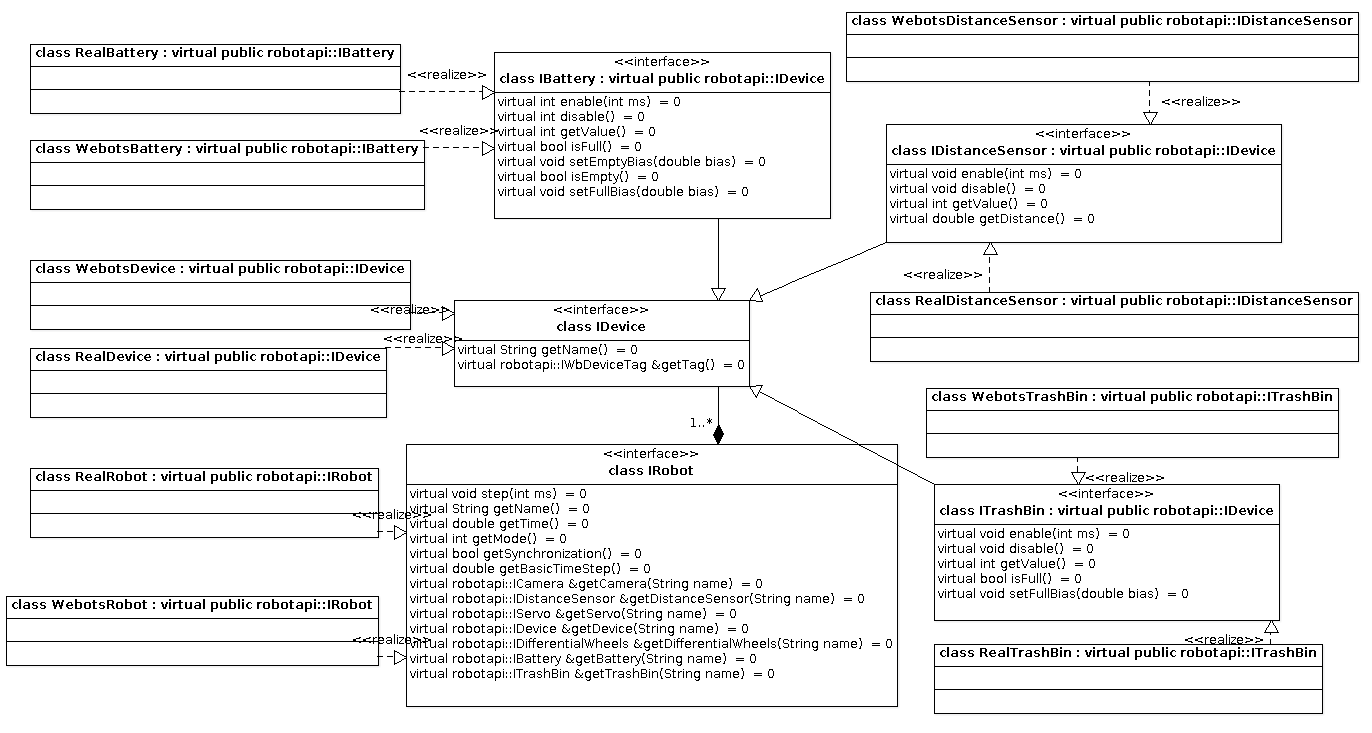
\includegraphics[scale=0.5]{comportamientos/figures/api2.png}
	\caption[Arquitectura de software: api de robot]{Diagrama de clases de la arquitectura
			de sofware. Paquete de api de l robot}
	\label{fig:soft_arq_devices}
\end{figure}
\end{landscape}

\subsection{Reconocimiento de objetos}
La figura \ref{fig:soft_arq_reconmodule} exhibe la relaci\'on entre el m\'odulo de reconocimiento de 
objetos y el m\'odulo de comportamientos. El m\'odulo de visi\'on queda encapsulado dentro
de la clase de \textit{GarbageRecognition}, permitiendo que el m\'odulo de comportamientos funcione en
forma independiente a \'este. La creaci\'on de una interface para la c\'amara nos permite alternar
entre el entorno de webots y el mundo real. El comportamiento de las clases \textit{WebotsCamera} y 
\textit{RealCamera} es el mismo pero sus implementaci\'ones difieren en que, en el caso de la primera, se pide
la imagen a webots mientras
que en la segunda se toma una imagen del mundo real. Por motivos similares utilizamos una interface para 
la representaci\'on de las im\'agenes.\'Esto se debe a que OpenCV y Webots codifican las im\'agenes de
maneras distintas y tuvimos que implementar sus respectivas clases. 
\begin{landscape}
\begin{figure}[h]
	\centering
	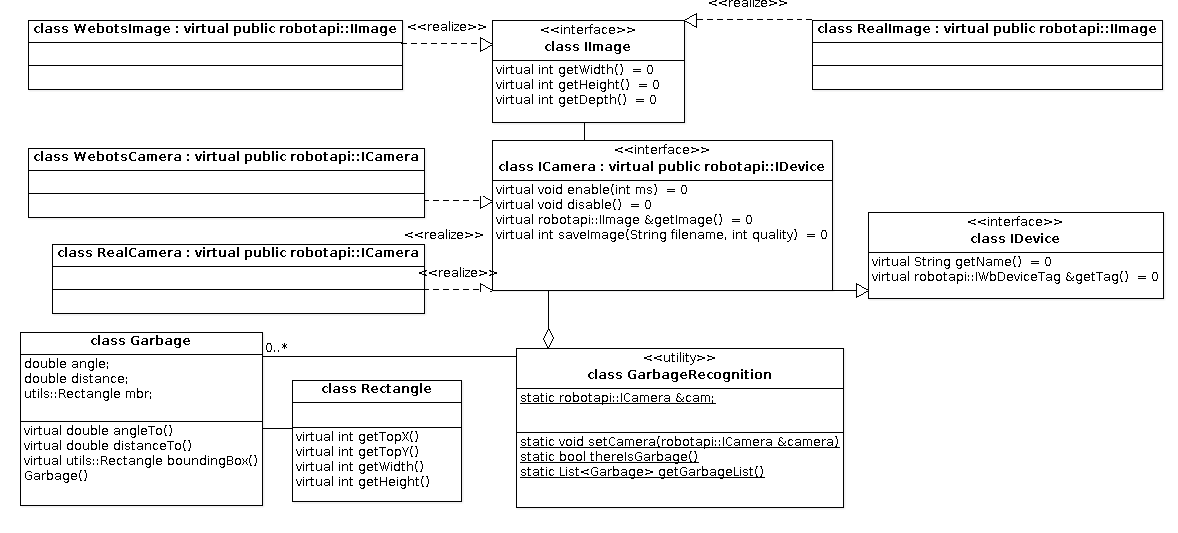
\includegraphics[scale=0.5]{comportamientos/figures/api3.png}
	\caption[Arquitectura de software: m\'odulo de reconocimiento]{Diagrama de clases de
	la arquitectura de software. Paquete de reconocimiento de basuras}
	\label{fig:soft_arq_reconmodule}
\end{figure}
\end{landscape}

\section[Implementaci\'on del protocolo en PC]{Implementaci\'on del protocolo de comunicaci\'on del lado de la PC}
\subsection{Packet Server}
La implementaci\'on del protocolo en la PC la hicimos en C++, al igual que
el controlador y el m\'odulo de reconocimiento de basuras. Para la misma
implementamos los paquetes descriptos en el protocolo y un servidor de
env\'io y recepci\'on de los mismos a trav\'es del puerto serial. Tambi\'en
implementamos lo que llamamos handlers, quienes son los responsables de
convertir los comandos de la api del robot en paquetes y enviarlos al
servidor, as\'i como tambi\'en de recibir los paquetes de respuesta que
le incumben y proveerlos a la api de una forma que \'esta los entienda.
Mostramos el diagrama de \'esta relaci\'on en la figura
\ref{fig:diag_server_handler_packet}.
\\\indent
Como mencionamos anteriormente, hay un servidor que denominamos packet
server encargado del env\'io y recepci\'on de paquetes. El servidor s\'olo
se encarga de mandar una serie de bytes y de recibir los mismos, sin
inspeccionar de qu\'e tipo de paquete se trata. Provee
dos m\'etodos para realizar el env\'io y recepci\'on:
\begin{itemize}
	\item{sendPacket:} Su funci\'on es recibir un paquete y encolarlo para
		que el servidor lo env\'ie. Como el servidor es un thread diferente
		al de la api, no se interrumpe la recepci\'on o env\'io de paquetes.
	\item{registerHandler:} Registra un handler para un paquete enviado desde
		una placa con grupo $groupid$ e id de placa $boardid$. Cuando llega
		un paquete de dicha placa, el servidor invoca el m\'etodo
		handlePacket() del handler registrado.
\end{itemize}
La idea del m\'etodo handlePacket es que se limite s\'olo a guardar los
nuevos valores recibidos, ya que durante la invocaci\'on del mismo el
server no recibe ni env\'ia paquetes.
La clase packet provee funciones de utilidad para cualquier tipo de
paquete, tales como c\'alculo y verificaci\'on de CRC, seteo y obtenci\'on
de valores de los campos del paquete, entre otras.
\begin{figure}[ht]
	\centering
	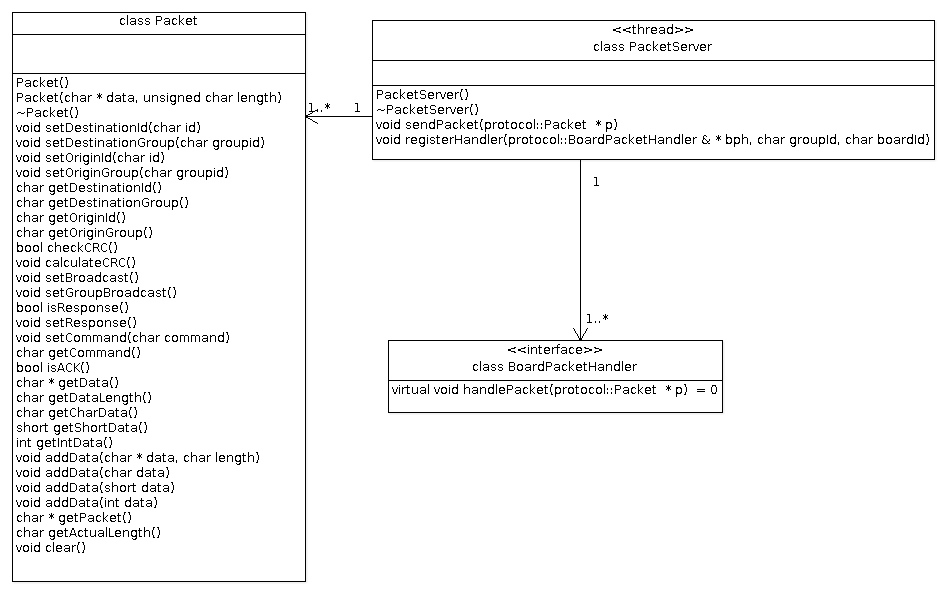
\includegraphics[scale=0.483]{comportamientos/figures/cs4.png}
	\caption[Diagrama de clases: Servidor de paquetes e interface]
			{Diagrama de clases. Estructura general del servidor de paquetes
			e interface para los handlers.}
	\label{fig:diag_server_handler_packet}
\end{figure}
\subsection{Packets}
Como indicamos en la figura \ref{fig:packet_group_board}, group packet extiende
a packet, agreg\'ando m\'etodos de utilidad para los comandos que todos
los grupos son capaces de recibir. Lo mismo sucede con board packet,
extendiendo de group packet ya que es m\'as espec\'ifico que este \'ultimo.

\begin{figure}[ht]
	\centering
	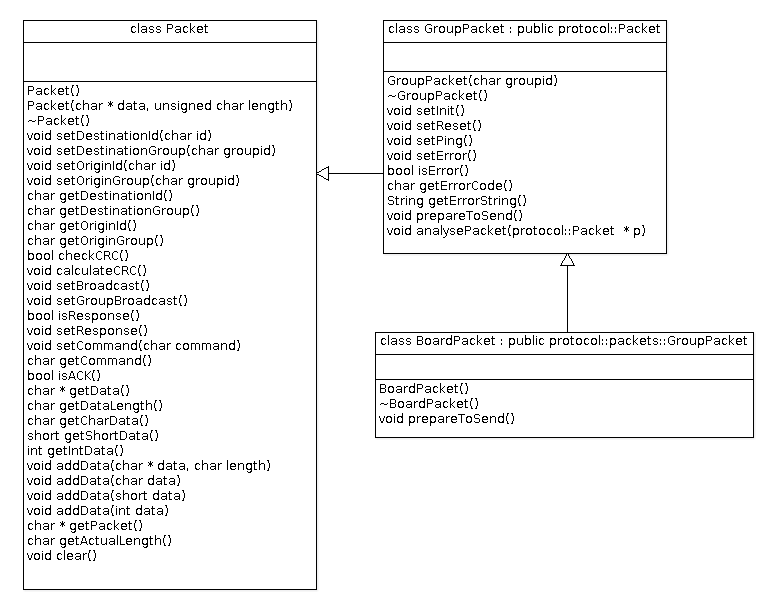
\includegraphics[scale=0.5]{comportamientos/figures/cs1.png}
	\caption[Diagrama de clases: Estructura general]{Diagrama de clases. Estructura general de los paquetes.}
	\label{fig:packet_group_board}
\end{figure}

En las figuras \ref{fig:packet_specific_1} y \ref{fig:packet_specific_2}
mostramos los paquetes que extienden de board packet, espec\'ificos para
cada sensor o actuador que pueda haber en una placa. Como se puede observar,
cada paquete espec\'ifico tiene funciones que permiten obtener y setear
informaci\'on propia del sensor/actuador en cuesti\'on, respetando el
protocolo que propusimos.
\\\indent
Por ejemplo, BatteryPacket permite setear los thresholds o
umbrales a los cuales informar\'a que la bater\'ia se encuentra cargada o
en estado cr\'itico, respectivamente. Adem\'as permite obtener el valor
de carga de la bater\'ia.
\\\indent
A continuaci\'on damos un ejemplo de uso de un paquete. Supongamos que se
quiere saber la carga de la bater\'ia. Para \'esto instanciamos un
BatteryPacket con el id de grupo y placa correspondientes. El mismo se
encarga del seteo de los campos de grupo y placa de origen y destino,
tama\~no del paquete y comando. Le indicamos que queremos el valor de carga
con senseBattery(), que pone el comando correspondiente en el campo del
paquete. Una vez que tenemos el paquete armado, llamamos a la funci\'on
sendPacket() del packet server. Suponiendo que registramos un handler para
ese id de grupo y de placa, cuando el server reciba la respuesta de la placa
va a llamar al m\'etodo handlePacket() del handler. En la funci\'on,
instanciamos un BatteryPacket y llamamos a la funci\'on analysePacket()
con el paquete que recibimos. Finalmente, nos queda invocar al m\'etodo
getBatteryValue() de este paquete.

\begin{figure}[ht]
	\centering
	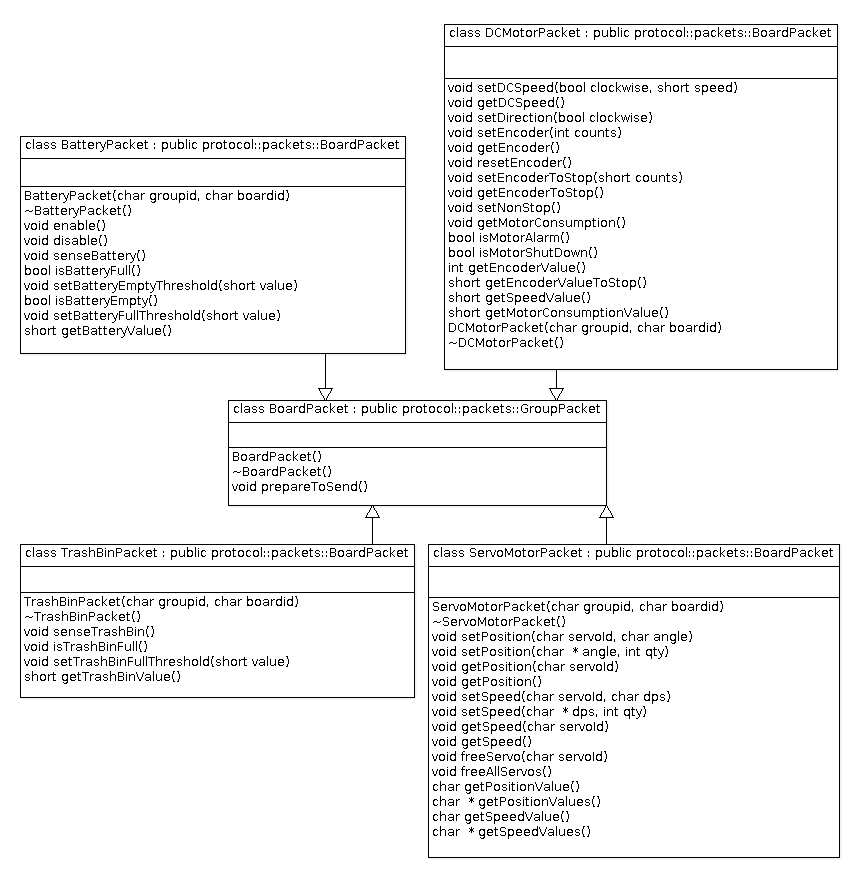
\includegraphics[scale=0.52]{comportamientos/figures/cs2.png}
	\caption[Diagrama de clases: Estructura paquetes 1]{Diagrama de clases. Estructura de los paquetes de motor, recipiente de basura, servos y bater\'ia.}
	\label{fig:packet_specific_1}
\end{figure}

\begin{figure}[ht]
	\centering
	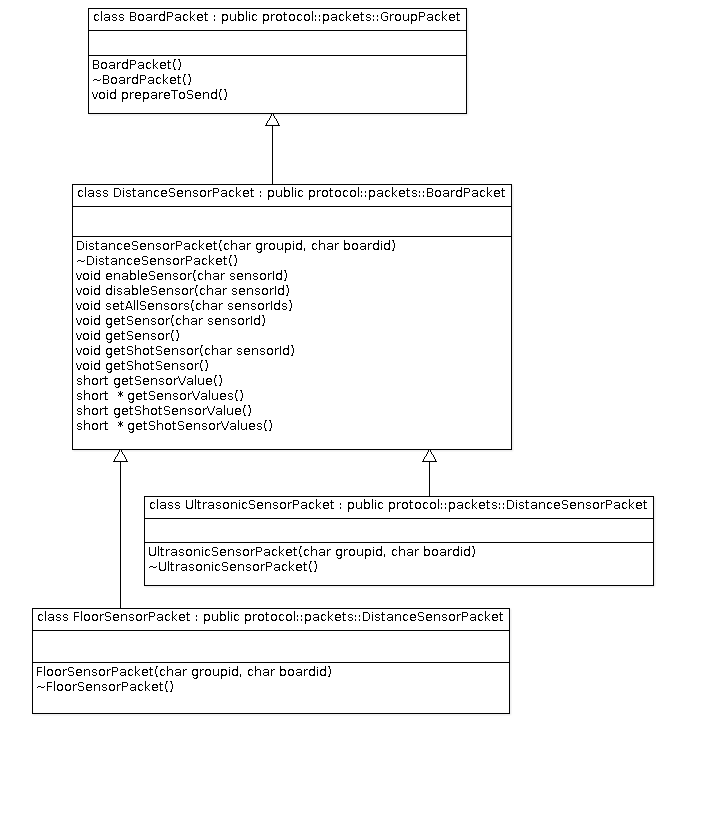
\includegraphics[scale=0.52]{comportamientos/figures/cs3.png}
	\caption[Diagrama de clases: Estructura paquetes 2]{Diagrama de clases. Estructura general de los paquetes para sensores de distancia.}
	\label{fig:packet_specific_2}
\end{figure}

\subsection{Handlers}
En las figuras \ref{fig:handler_specific_1} y \ref{fig:handler_specific_2}
mostramos los handlers implementados para que las implementaciones de los
sensores de la api del robot pudieran manejar los mismos, sin tener
conocimiento sobre el protocolo. Hay un handler por default,
DefaultBoardPacketHandler, para el caso en que no haya registrado un handler
para determinado id de grupo y placa. La funci\'on handlePacket del mismo
se encarga de imprimir por salida est\'andar cada campo del paquete en
formato hexadecimal.
\\\indent
Se puede observar que la cantidad de m\'etodos en los paquetes y en los
handlers no es la misma, y en algunos casos, hay m\'etodos que en el otro
no est\'an. \'Esto se debe a que los handlers son intermediarios entre
el protocolo y la api del controlador encargado de la ejecuci\'on de los
comportamientos. En algunos casos, el protocolo brinda m\'as opciones de
las que realmente utiliza el controlador para funcionar.
\begin{figure}[ht]
	\centering
	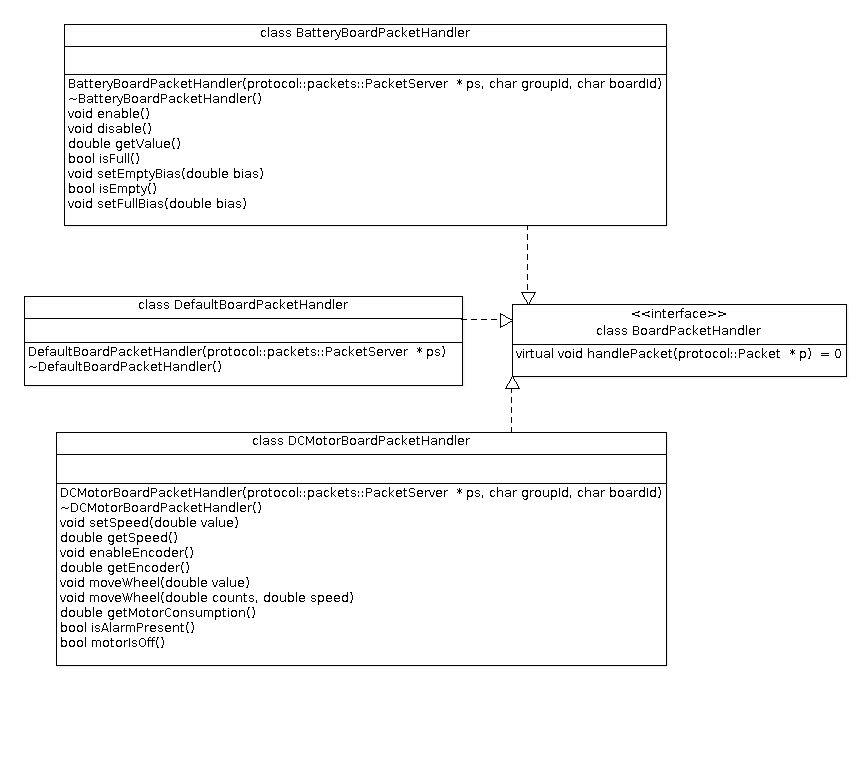
\includegraphics[scale=0.5]{comportamientos/figures/cs5.png}
	\caption[Diagrama de clases: Handlers 1]{Diagrama de clases. Handlers de paquetes default y para las placas de motor y 
	bater\'ia.}
	\label{fig:handler_specific_1}
\end{figure}

\begin{figure}[ht]
	\centering
	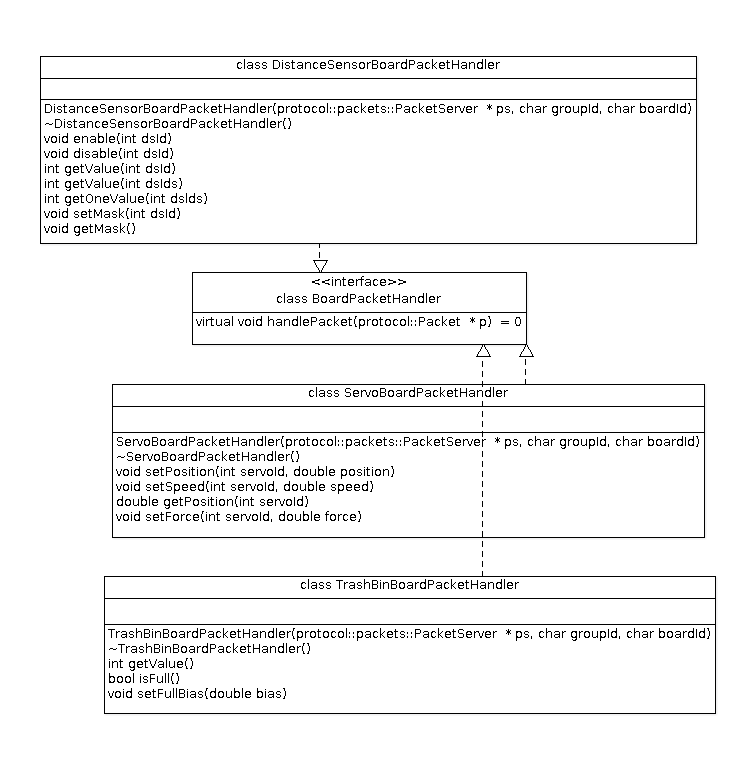
\includegraphics[scale=0.52]{comportamientos/figures/cs6.png}
	\caption[Diagrama de clases: Handlers 2]{Diagrama de clases. Handlers de paquetes para las placas de sensores de 
	distancia, servos y recipiente de residuos.}
	\label{fig:handler_specific_2}
\end{figure}


\subsection{Qu\'e hacer en caso que se modifique el protocolo}
En el caso que haya una modificaci\'on en el protocolo, se deber\'an
actualizar las clases afectadas por los cambios, y eventualmente,
los handlers correspondientes.
\\\indent
Supongamos el caso en el que se agrega un campo de 1 byte luego del tama\~no
total del paquete. \'Este cambio, en principio, s\'olo afecta la clase
Packet. En el caso que el campo indique algo sobre el grupo o placa,
tambi\'en afectar\'a a group packet o board packet, respectivamente.
En el caso que se ampl\'ie el set de comandos de un determinado sensor o
actuador, es necesario modificar el packet y handler asociados a los
mismos. Lo importante de \'esto es que los cambios est\'an localizados.
Es decir, un cambio en el protocolo llega como mucho hasta los handlers,
aislando a la api del controlador de posibles cambios.





